\chapter{Analysis of Results from the Core Model} \label{chapter-analysis}


\section{The baseline model} 
The two main hypotheses of this thesis are, first,  that the financial sector affects the ownership of housing and the class structure of society, and second that this may have implications for urban productivity. We begin with the first hypothesis.

\section{ownership of housing}

Our baseline model, described in detail elsewhere, produces an evolutionary trajectory of class ownership of housing illustrated in Figure ~\ref{fig:Baseline_ownership_trajectory}. Recall that our first hypothesis is that in and \Gls{Alonzo-Jacobs model}, the financial sector will take over a growing share of property ownership within a city. Figure ~\ref{fig:Baseline_ownership_trajectory} shows an initial situation with close to 100 owner-occupiers and a small number of investor-owners. Although the number of owner-occupiers grows in the initial period but, over time, financial capital acquires an increasing share of the housing stock. By the time the city reaches its maximum size, the city has been transformed from a city of homeowners to a city of tenants.  

\begin{figure}
    \centering
    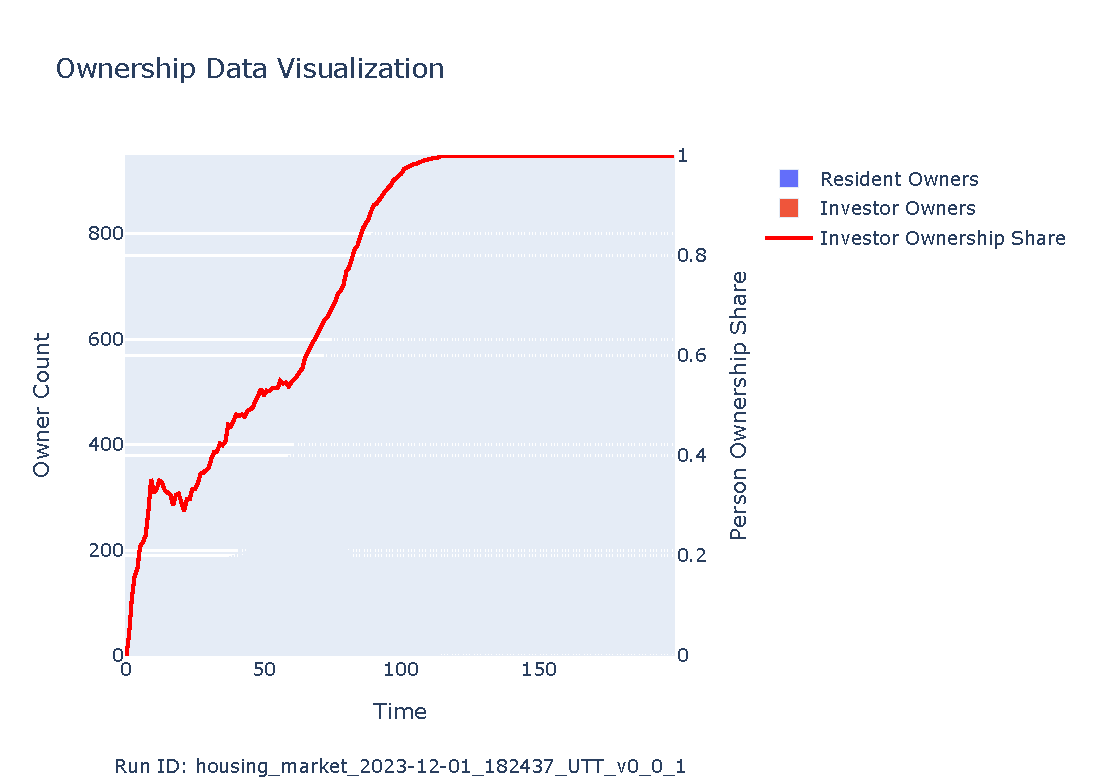
\includegraphics[scale=.8, trim={0 1cm 0 1.8cm},clip]{fig/Analysis/Ownership_Data_1.pdf}
    \caption{The transformation from a city of homeowners to a city of tenants in the baseline model}
    \label{fig:Baseline_ownership_trajectory}
\end{figure}



Initially, 100\% of locational land rent accrues to residents. In the end, 100\% accrues to the owners of financial capital. Total rents at the end of the period of growth are six times their initial size. 
Initially, 100\% of locational land rent accrues to residents. In the end, 100\% accrues to the owners of financial capital. Total rents at the end of the period of growth are eight times their initial size.\footnote{Recall that the radius of a circular city is proportional to the wage premium. Rent can be visualized as a cone of volume $\pi r^2 h$ where $h$ is the wage premium. If we double $h$, the volume is increased by a factor of 8.}

 